\section{هوش مصنوعی و معماری کامپیوتر}
\begin{frame}{مقدمه}
\begin{itemize}\itemr
\item[-]
در دهه‌های ۸۰ و ۹۰ میلادی، کامپیوتر‌‌ها هر ۱۸ تا ۲۴ ماه (قانون مور) سریع‌تر می‌شدند.
\item[-]
این یعنی اگر شما امسال یک کامپیوتر می‌خریدید و دوستان شما یک سال بعد از شما کامپیوتر جدیدی می‌خریدند، کامپیوتر‌ آنها بسیار سریع‌تر می‌بود
\item[-]
اما امروزه، تنها راه پیشرفت در معماری کامپیوتر ساخت سخت‌افزار برای یک کاربرد خاص است.
\item[-]
برای مثال پردازند‌ه‌ها گرافیکی
\lr{(GPU)}
برای انجام محاسبات گرافیکی بسیار کارامد هستند. آنها می‌توانند میلیون‌ها ضرب ماتریس در یک هر ثانیه انجام بدهند.
\end{itemize}
\end{frame}

\begin{frame}{پردازنده‌ی \lr{TPU}}
\begin{itemize}\itemr
\item[-]
با رخ دادن انقلابی در هوش مصنوعی به نام \textbf{یادگیری ماشین} که به ضرب ماتریسی متکی بود، نیاز به پردازنده‌های مخصوص ضرب تانسور‌ها برای اجرا سریع‌تر و دقیق‌تر الگوریتم‌ها یادگیری ماشین احساس می‌شد،
\item[-]
واحد پردازش تانسور
\lr{(Tensor Processing Unit (TPU))}
شتاب‌دهنده‌ی یادگیری ماشین است که توسط گوگل طراحی شده است. 
\lr{TPU}ها
برای ضرب ماتریس‌ها بسیار کارامند هستند که برای آموزش شبکه‌های عصبی 
\lr{ANN}
ضروریست.
\end{itemize}
\end{frame}

\begin{frame}{طراحی سطح بالا}
\begin{center}
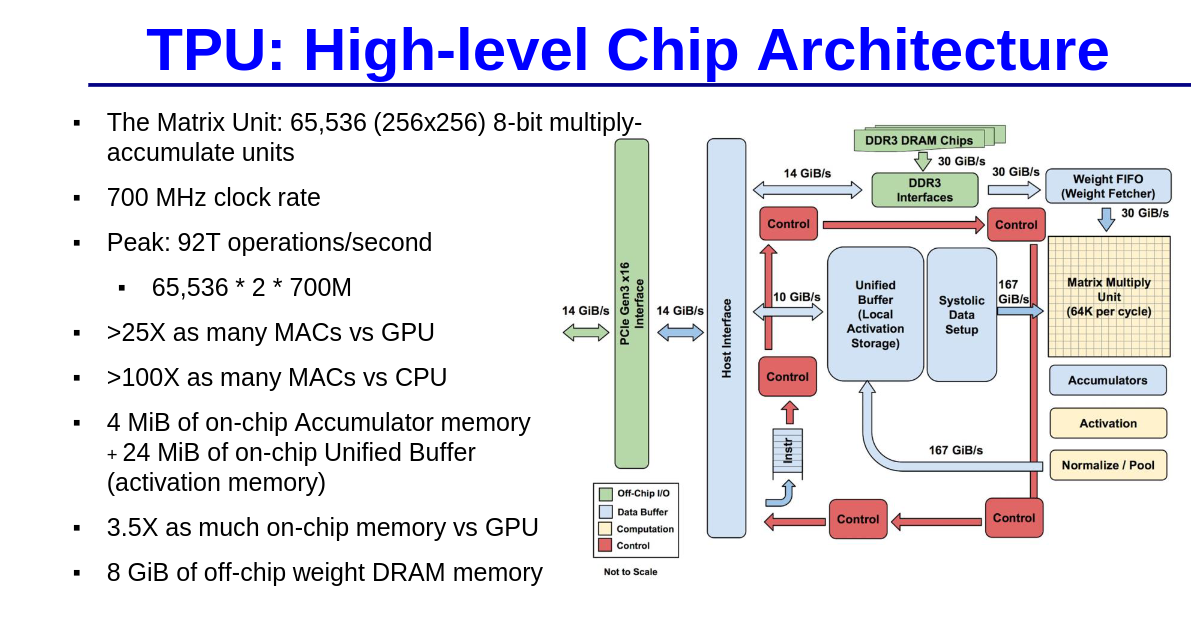
\includegraphics[width=0.9\textwidth, height=0.8\textheight]{docs/images/tpu-1}
\end{center}
\end{frame}

\begin{frame}{کارایی/توان مصرفی}
\begin{center}
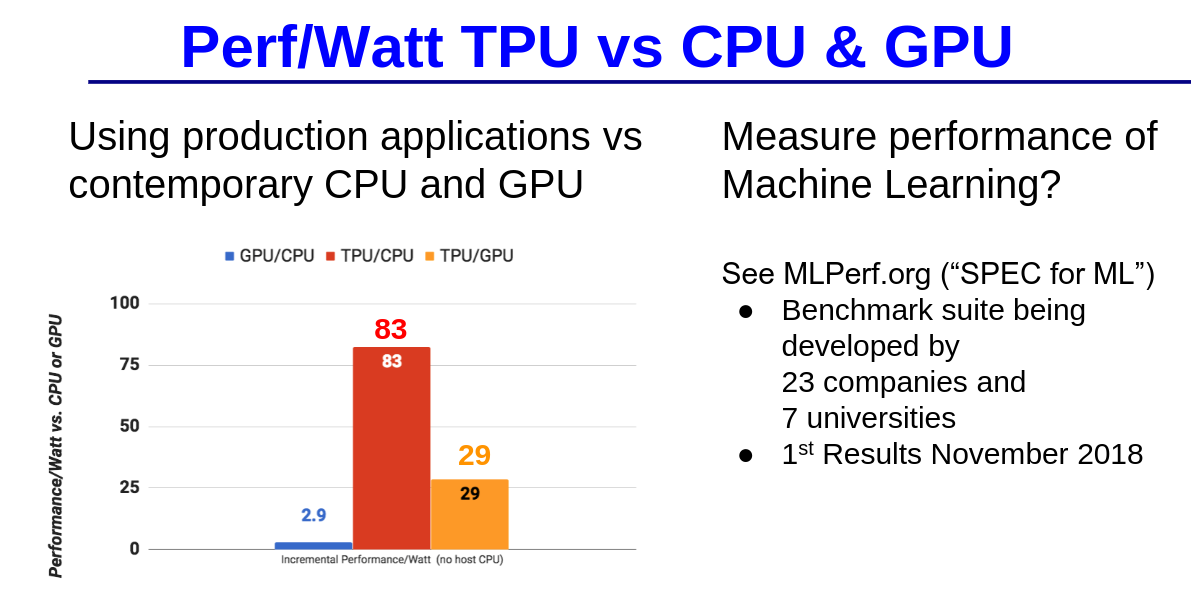
\includegraphics[width=0.9\textwidth, height=0.8\textheight]{docs/images/tpu-2}
\end{center}
\end{frame}
